\section{Hyperbolic Equation System}
In the simulatin of partial melting system, 
there arises multidimensional hyperbolic equations systems.
\begin{equation}
		  \bold{U}_t + \nabla \cdot [F(\bold{U}) - \mathcal{D}\nabla \bold{U}] = 0
\end{equation}
$\bold{U}$ consists of two variables, average concentration of one species $\bar{c}_1$ and 
average total internal energy $\bar{E}$.
\begin{equation}
		  \begin{aligned}
					 c_t + \nabla \cdot (\bold{v}^c_e c - \kappa D \nabla c) &= 0\\
					 H_t + \nabla \cdot (\bold{v}^H_e H - \bar{K}\nabla T) &= 0
		  \end{aligned}
\end{equation}
where 
\begin{equation}
		  \nabla T(c, H) = \frac{\partial T}{\partial c} \nabla c + \frac{\partial T}{\partial H} \nabla H 
\end{equation}
The diffusive matrix $\mathcal{D}$ can be rewritten as:
\begin{equation}
		  \mathcal{D} = \begin{bmatrix}
        \kappa D & 0 \\
					 \bar{K} \frac{\partial T}{\partial c} & \bar{K} \frac{\partial T}{\partial H}
		  \end{bmatrix}
\end{equation}
Corresponding solid and liquid velocities are determined by solving the degenerate Darcy-Stokes system proposed above.
Let's take a closer look on the coupled diffusive matrix $\mathcal{D}$, partial derivatives of temperature against 
composition and enthalpy requires calculation.
We can get those partial derivatives directly from phase package where relationship between temperature and compostion and enthalpy
are expressed explicitly.
We can approximate the partial derivative matrix with a diagonal matrix, that is, $\frac{\partial T_i}{\partial c_j} = \left \{ \begin{aligned} 
		  0 &\quad i\neq j\\
		  f(c,H) & \quad i = j
\end{aligned} \right.$. 

\subsection{Calculation of $\kappa$}
where $\kappa = \frac{\phi_f c_f}{\bar{c}}$ need definition on edge shared between two cells.
\begin{center}
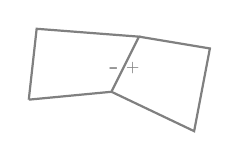
\begin{tikzpicture}
		  \draw[gray,thick] (-0.2,0.1) -- (0.85,0.2) -- (1.2,0.9) -- (-0.1,1) -- (-0.2,0.1);
		  \draw[gray,thick] (0.85,0.2) -- (1.9,-0.3) -- (2.1,0.75) -- (1.2,0.9);
		  \draw[gray] (0.7,0.5) node[anchor=west] {-};
		  \draw[gray,thick] (0.9,0.5) node[anchor=west] {\tiny +};
\end{tikzpicture}
\end{center}
There are two $\kappa$ values defined on both sides of the shared edge.
\begin{equation*}
		  \kappa^{\pm} = \frac{\phi_f c^{\pm}_f}{\bar{c}^{\pm}}
\end{equation*}
where $\phi_f$ has definition on the edge.

\subsection{Algorithms and flux}


\subsection{Notes}
Difficulties in solving transport system involving melting:
\begin{itemize}
\item Partial melting creates irregular porosity distribution.
Need small stencils accounting for complex situation, which leads to the development of multi-level WENO.
\end{itemize}
A new multi-level weno algorithm has beed developed\cite{MultiLevelWeno}.
Details regarding calculation of nonlinear weighting and jacobian for implicit time stepping are presented as follows.
